\chapter{Addestramento rete neurale}\label{addestramento-rete-neurale}


Come già menzionato nei capitoli precedenti l’idea è quella di allenare una \gls{cnn} per la classificazione dei frame di una laringoscopia attraverso il transfer learning impiegando la tecnica del
fine-tuning nelle due varianti (One Round Tuning e Two Round Tuning)  su una rete pre-allenata chiamata AlexNet.

\section{AlexNet}\label{alexnet}
AlexNet è la rete che ha rivoluzionato la computer vision nel 2012 essa è una \gls{cnn} sviluppata
da Goffrey Hinton e Alex Krizhevsky dell’università di Toronto vince, con ampio margine, 
l’ImageNet challenge: object classification and detection su milioni di immagini e 1000 classi.

La rete AlexNet è organizzata nel seguente modo: costituita da 8 livelli di cui 5 di \gls{Convolution Layer} e 3 \gls{fully-connected}, ed infine la funzione
di attivazione \gls{ReLu}, la dimensione delle immagini in input è di \(227\times 227\). L'architettura completa con le dimensioni dei layer di \gls{convoluzione} è illustrata in \cref{fig:alexnet}\cite{alexnet}.  

\begin{figure}[ht]
    \centering
    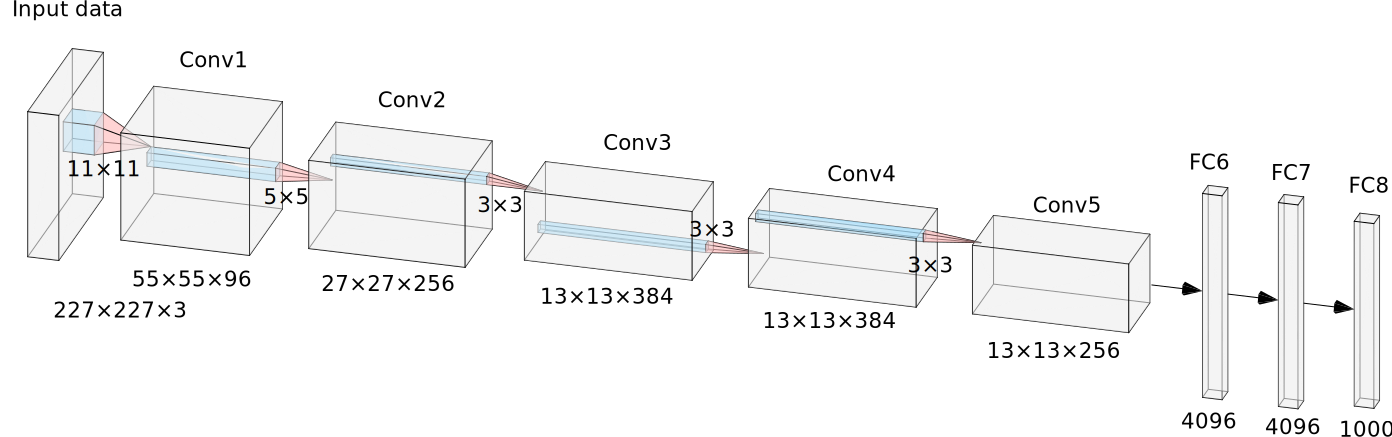
\includegraphics[width=0.7\textwidth]{addestramento-rete-neurale/alexnet.png}
    \caption{Architettura della \gls{cnn} AlexNet}
    \label{fig:alexnet}
\end{figure}

La rete AlexNet utilizzata è già allenata per il riconoscimento di 1000 classi di soggetti (mele, gatti, tastiere, telefoni, ecc.) su un dataset di oltre 1 milione di pattern presi dal database ImageNet\cite{alexnet}.

Viene usato un allenamento \(k\)-fold, in particolare con \(k=3\), in ogni fold i  pattern vengono elaborati con un
ordine diverso e si utilizza circa il 20\% di essi come test set.

\section{Allenamento 1R}\label{allenamento-1r}

La sperimentazione inizia con l'allenamento della \gls{cnn} con un fine-tuning standard e classico (denominato anche One Round Tuning, descritto in \cref{one-round-tuning}), nel senso che si rimpiazzano gli ultimi 3 layer e poi si riallena la rete. Come dataset è stato usato il dataset descritto NBI-InfFrames in \cref{descrizione-dei-dataset}. È da prestare attenzione ai vari iperparametri, come \Gls{LearningRate} e \Gls{MiniBatchSize}. In particolare è stato usato un learning rate di 0.0001 e un mini batch size di 30, il metodo di ottimizzazione è lo \gls{sgd}, come data augmentation sono stati usati i valori descritti nel \cref{data-augmentation}, in questo caso non è stata usata la discrete cousene transform. La confusion matrix di questo allenamento è mostrato in \cref{fig:one-liscio}.


\begin{figure}[ht]
    \centering
    \includegraphics[width=0.45\textwidth]{addestramento-rete-neurale/one-liscio.pdf}
    \caption{Confusion matrix dell'allenamento con TL 1R senza preprocessing e con una semplice data augmentation}
    \label{fig:one-liscio}
\end{figure}

\section{Allenamento 2R}\label{allenamento-2r}

L'allenamento 2R descritto in \cref{two-round-tuning} è composto da una prima fase di allenamento con un dataset similare e poi il dataset NBI-InfFrames, entrambi descritti in  \cref{descrizione-dei-dataset}. In questo caso gli iperparametri sono:   learning rate di 0.0001 e un mini batch size di 30, il metodo di ottimizzazione è il \gls{sgd}, come data argumentation sono stati usati i valori descritti nel \cref{data-augmentation} e non è stata usata la discrete cousene transform. La confusion matrix di questo allenamento è mostrato in \cref{fig:two-liscio}.


\begin{figure}[ht]
    \centering
    \includegraphics[width=0.45\textwidth]{addestramento-rete-neurale/two-liscio.pdf}
    \caption{Confusion matrix dell'allenamento con TL 2R senza preprocessing e con una semplice data augmentation}
    \label{fig:two-liscio}
\end{figure}

Per effettuare un allenamento 2R è sufficiente duplicare il codice di un TL facendo attenzione a usare la stessa rete.

\section{Image preprocessing}\label{image-preprocessing}

Un primo filtro di image preprocessing è modificare il contrasto dell'immagine, come noto il contrasto di una immagine influenza molto la vista umana, e dato che le \gls{cnn} sono molto simili al modello di connettività dei neuroni nel cervello umano è plausibile che modifiche al contrasto influenzano i risultati  ottenuti. Un semplice filtro per il contrasto si ottiene con:
\begin{lstlisting}
IM=imadjust(IM,[.2 .3 0; .6 .7 1],[]);    
\end{lstlisting}

In figura \cref{fig:contrast} sono presenti le confusion matrix dei risultati ottenuti con la modifica del contrasto.

\begin{figure}[ht]
    \centering
    \begin{subfigure}{0.45\textwidth}
        \includegraphics[width=\textwidth]{addestramento-rete-neurale/one-contrast.pdf}
        \caption{Allenamento 1R} 
    \end{subfigure}
    \begin{subfigure}{0.45\textwidth}
        \includegraphics[width=\textwidth]{addestramento-rete-neurale/two-contrast.pdf}
        \caption{Allenamento 2R} 
    \end{subfigure}
    \caption{Confusion matrix dell'allenamento con TL 1R e 2R con correzzione contrasto hardcoded}
    \label{fig:contrast}
\end{figure}

Dato che nella preelaborazione precedente si usa un filtro hardcoded, lo step successivo è modificare il  contrasto in base alla media e alla derivazione standard dell'immagine, con \lstinline{n} un iperparametro che indica quanto modificare il contrasto. In \cref{fig:contrast-bis}  la confusion matrix con i risulati ottenuti con una correzione contrasto dinamica.
\begin{lstlisting}
n = 0.5;  
Idouble = im2double(IM); 
avg = mean2(Idouble);
sigma = std2(Idouble);
IM = imadjust(IM,[avg-n*sigma avg+n*sigma],[]);
\end{lstlisting}

\begin{figure}[ht]
    \centering
    \begin{subfigure}{0.45\textwidth}
        \includegraphics[width=\textwidth]{addestramento-rete-neurale/one-contrast-bis.pdf}
        \caption{Allenamento 1R} 
    \end{subfigure}
    \begin{subfigure}{0.45\textwidth}
        \includegraphics[width=\textwidth]{addestramento-rete-neurale/two-contrast-bis.pdf}
        \caption{Allenamento 2R} 
    \end{subfigure}
    \caption{Confusion matrix dell'allenamento con TL 1R e 2R con correzione contrasto dinamica}
    \label{fig:contrast-bis}
\end{figure}

Una versione più avanzata per l'elaborazione del contrasto è il CLAHE

\begin{lstlisting}
[X, MAP] = rgb2ind(IM, 65536);
RGB = ind2rgb(X,MAP);
LAB = rgb2lab(RGB);
L = LAB(:,:,1)/100;
L = adapthisteq(L,'NumTiles',[8 8],'ClipLimit',0.005);
LAB(:,:,1) = L*100;
IM = lab2rgb(LAB);
\end{lstlisting}

\begin{lstlisting}
IM = imnoise(IM,'salt & pepper',0.02);
\end{lstlisting}

\begin{lstlisting}
IM= hgamma(IM);
\end{lstlisting}

\section{Data argumentation con DCT}\label{data-argumentation-con-dct}





\section{Ensemble di classificatori}\label{ensemble-di-classificatori}

